% !TEX root = ../thesis.tex

\section{Basic Definitions and Results}\label{sec:preliminaries}
In this section we introduce some basic definitions and results that are used throughout this thesis.
We start with some preliminaries on hypergraphs, which are the main objects of study in this thesis.

\subsection{Hypergraphs}\label{subsec:hypergraphs}

\begin{definition}

    For an integer $k \geq 1$ a finite \emph{$k$-uniform hypergraph} (or \emph{$k$-graph}, for short)
    is a tuple $G = (V, E)$ where $V$ is a finite set
    and $E \subset \binom{V}{k}$.
    We call the elements of $V(G) = V$ its \emph{vertices}
    and those of $E(G) = E$ its \emph{edges}.
    The value $k$ is called the \emph{uniformity} of $G$.
\end{definition}

\begin{remark}
    In the definition above, if we let $k=1$ we get a set of $1$-sets of the vertex set $V$,
    which we can identify with a subset of $V$.
    If we let $k=2$ we recover the usual definition of an undirected graph with no loops.
\end{remark}

The following definition is a generalization of the notion of degree
of a vertex in a graph.

\begin{definition}
    Let $G = (V, E)$ be a $k$-graph and $v \in V$.
    The \emph{degree} $d_G(v)$ of $v$ in $G$
    is the number of edges containing $v$, that is
    \[
        d_G(v) = |\{e \in E \mid v \in e\}|.
    \]
\end{definition}

A useful operation is restricting a k-graph to a subset of its vertices.
This yields a new k-graph, called the \emph{subgraph induced by} the subset, which has the same uniformity.

\begin{definition}

    \label{def:restriction}
    Let $G = (V, E)$ be a $k$-graph and $T \subset V$.
    The \emph{restriction} of $G$ to $T$ is the $k$-graph
    \[
        G[T] = (T, E_T),
    \]
    where
    \[E_T = \{e \in E \mid e \subset T\}.\]
\end{definition}

The following operation also lets us obtain graphs of a
different uniformity from a subset of vertices of a $k$-graph.

\begin{definition} \label{def:link}
    Let $G = (V, E)$ be a $k$-graph.
    Let $1 \leq j \leq k - 1$ be an integer and let
    $T \subset V$ be a set of vertices satisfying $k - j \leq |T|$.
    The \emph{common $j$-link graph} of $T$ is the $j$-graph $\link{G}{T}{j} = (V \setminus T, E')$, where
    \[
        E' = \left\{Y \in \binom{V}{j}\middle\vert \, X \cup Y \in E \text{ for all } X \in \binom{T}{k-j}\right\}.
    \]
\end{definition}

\begin{figure}[htbp]
    \centering
    % TikZ code generated by Python script for Common Link Graph visualization
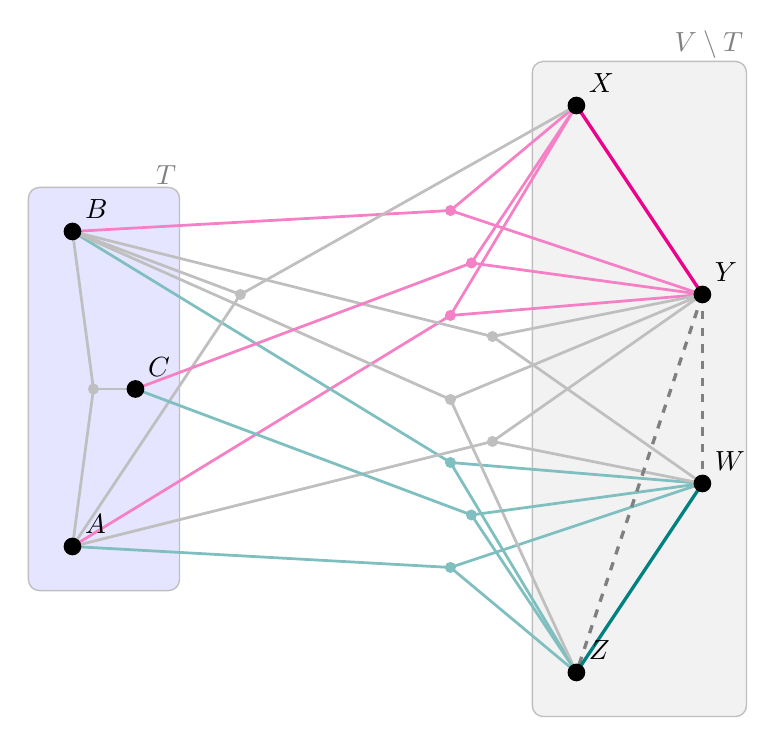
\begin{tikzpicture}[scale=0.8]
% Vertex coordinates
\coordinate (A) at (0.00, 2.00);
\coordinate (B) at (0.00, 7.00);
\coordinate (C) at (1.00, 4.50);
\coordinate (X) at (8.00, 9.00);
\coordinate (Y) at (10.00, 6.00);
\coordinate (Z) at (8.00, 0.00);
\coordinate (W) at (10.00, 3.00);
% Hyperedge root coordinates
\coordinate (R0) at (6.000, 5.667);
\coordinate (R2) at (6.000, 7.333);
\coordinate (R3) at (6.667, 5.333);
\coordinate (R4) at (6.000, 1.667);
\coordinate (R5) at (6.000, 3.333);
\coordinate (R6) at (2.667, 6.000);
\coordinate (R7) at (6.667, 3.667);
\coordinate (R8) at (6.000, 4.333);
\coordinate (R9) at (0.333, 4.500);
\coordinate (R10) at (6.333, 6.500);
\coordinate (R11) at (6.333, 2.500);
% Draw background boxes for T and V \ T
\draw[fill=blue!10, rounded corners, line width=0.5pt, draw=gray!50] (-0.70, 1.30) rectangle (1.70, 7.70);
\node at (1.70, 7.70) [anchor=south east, inner sep=1pt, text=gray] {$T$};
\draw[fill=gray!10, rounded corners, line width=0.5pt, draw=gray!50] (7.30, -0.70) rectangle (10.70, 9.70);
\node at (10.70, 9.70) [anchor=south east, inner sep=1pt, text=gray] {$V \setminus T$};
% Draw original hyperedges (styled by category)
\draw[line width=1.0pt, color=magenta!50!white, solid] (R0) -- (A);
\draw[line width=1.0pt, color=magenta!50!white, solid] (R0) -- (X);
\draw[line width=1.0pt, color=magenta!50!white, solid] (R0) -- (Y);
\fill[magenta!50!white] (R0) circle (2.5pt);
\draw[line width=1.0pt, color=magenta!50!white, solid] (R2) -- (B);
\draw[line width=1.0pt, color=magenta!50!white, solid] (R2) -- (X);
\draw[line width=1.0pt, color=magenta!50!white, solid] (R2) -- (Y);
\fill[magenta!50!white] (R2) circle (2.5pt);
\draw[line width=1.0pt, color=gray!50!white, solid] (R3) -- (B);
\draw[line width=1.0pt, color=gray!50!white, solid] (R3) -- (Y);
\draw[line width=1.0pt, color=gray!50!white, solid] (R3) -- (W);
\fill[gray!50!white] (R3) circle (2.5pt);
\draw[line width=1.0pt, color=teal!50!white, solid] (R4) -- (A);
\draw[line width=1.0pt, color=teal!50!white, solid] (R4) -- (Z);
\draw[line width=1.0pt, color=teal!50!white, solid] (R4) -- (W);
\fill[teal!50!white] (R4) circle (2.5pt);
\draw[line width=1.0pt, color=teal!50!white, solid] (R5) -- (B);
\draw[line width=1.0pt, color=teal!50!white, solid] (R5) -- (Z);
\draw[line width=1.0pt, color=teal!50!white, solid] (R5) -- (W);
\fill[teal!50!white] (R5) circle (2.5pt);
\draw[line width=1.0pt, color=gray!50!white, solid] (R6) -- (A);
\draw[line width=1.0pt, color=gray!50!white, solid] (R6) -- (B);
\draw[line width=1.0pt, color=gray!50!white, solid] (R6) -- (X);
\fill[gray!50!white] (R6) circle (2.5pt);
\draw[line width=1.0pt, color=gray!50!white, solid] (R7) -- (A);
\draw[line width=1.0pt, color=gray!50!white, solid] (R7) -- (Y);
\draw[line width=1.0pt, color=gray!50!white, solid] (R7) -- (W);
\fill[gray!50!white] (R7) circle (2.5pt);
\draw[line width=1.0pt, color=gray!50!white, solid] (R8) -- (B);
\draw[line width=1.0pt, color=gray!50!white, solid] (R8) -- (Y);
\draw[line width=1.0pt, color=gray!50!white, solid] (R8) -- (Z);
\fill[gray!50!white] (R8) circle (2.5pt);
\draw[line width=1.0pt, color=gray!50!white, solid] (R9) -- (A);
\draw[line width=1.0pt, color=gray!50!white, solid] (R9) -- (B);
\draw[line width=1.0pt, color=gray!50!white, solid] (R9) -- (C);
\fill[gray!50!white] (R9) circle (2.5pt);
\draw[line width=1.0pt, color=magenta!50!white, solid] (R10) -- (C);
\draw[line width=1.0pt, color=magenta!50!white, solid] (R10) -- (X);
\draw[line width=1.0pt, color=magenta!50!white, solid] (R10) -- (Y);
\fill[magenta!50!white] (R10) circle (2.5pt);
\draw[line width=1.0pt, color=teal!50!white, solid] (R11) -- (C);
\draw[line width=1.0pt, color=teal!50!white, solid] (R11) -- (Z);
\draw[line width=1.0pt, color=teal!50!white, solid] (R11) -- (W);
\fill[teal!50!white] (R11) circle (2.5pt);
% Draw 'almost' link edges (faintly, dotted)
\draw[color=gray, very thick, dashed] (Y) -- (Z);
\draw[color=gray, very thick, dashed] (Y) -- (W);
% Edges of the common 2-link graph of T (brightly colored)
\draw[very thick, color=magenta] (X) -- (Y);
\draw[very thick, color=teal] (Z) -- (W);
% Draw vertices (foreground layer)
\fill[black] (A) circle (4.0pt);
\node[above right=1pt, color=black] at (A) {$A$};
\fill[black] (B) circle (4.0pt);
\node[above right=1pt, color=black] at (B) {$B$};
\fill[black] (C) circle (4.0pt);
\node[above right=1pt, color=black] at (C) {$C$};
\fill[black] (X) circle (4.0pt);
\node[above right=1pt, color=black] at (X) {$X$};
\fill[black] (Y) circle (4.0pt);
\node[above right=1pt, color=black] at (Y) {$Y$};
\fill[black] (Z) circle (4.0pt);
\node[above right=1pt, color=black] at (Z) {$Z$};
\fill[black] (W) circle (4.0pt);
\node[above right=1pt, color=black] at (W) {$W$};
\end{tikzpicture}
    \caption{A $3$-graph $G$ and the common $2$-link graph $\link{G}{T}{2}$ of the set $T = \{A, B, C\}$.
        The link graph has vertex set $\{X, Y, Z, W\}$ and edge set
        $\{\{X, Y\}, \{W, Z\}\}$.
    }
    \label{fig:link}
\end{figure}

Figure~\ref{fig:link} exemplifies how to construct
a common $j$-link graph from a $k$-graph $G$ in the case $k=3$ and $j=2$.
Vertices are represented as black dots, and $3$-edges of $G$ are represented as colored or gray small dots,
connected by a line to the vertices they contain.
Colored dots correspond to $3$-edges with exactly
$k - j = 3 - 2 = 1$ vertices in $T$, which are the only ones that can contribute to the common $2$-link graph.
Edges in the common $2$-link graph are represented as solid lines connecting the corresponding vertices,
in the same color that the $3$-edges they come from.
Dashed lines correspond to edge pairs
in $V \setminus T$ that have some of the required $3$-edges in $G$, but not all of them.

\begin{remark}
    Definition~\ref{def:link} might appear confusing because $E'$ is defined
    as a set of subsets of $V$, while the link graph has vertex set $V \setminus T$.
    In fact, it is impossible for an element $Y \in E'$ to contain a vertex $v \in T$.
    To see this, suppose that $v \in Y$.
    We can pick a $(k-j)$-set $X \in \binom{T}{k-j}$ such that $v \in X$.
    Then $v \in X \cup Y$ and
    $| X \cup Y | < j + (k-j) = k$, contradicting the fact that $X \cup Y$ is an edge in $G$.
\end{remark}

Next, we introduce $k$-graph homomorphisms, embeddings and isomorphisms, which allow us
to relate $k$-graphs of the same uniformity to each other.

\begin{definition} \label{def:embedding}
    Let $G = (V, E)$ and $H = (W, F)$ be $k$-graphs and let $f: V \to W$ be a map
    between their vertex sets.
    If $A \subset E$ is a set of edges in $G$, we denote
    \[
        f(A) = \{f(e) \mid e \in A\} = \{\{f(v) \mid v \in e\} \mid e \in A\}.
    \]
    Then, $f$ is a \emph{homomorphism} from $G$ to $H$ if
    \begin{equation}
        \label{eq:homomorphism}
        f(E) \subset E(H[f(V)]).
    \end{equation}
    If such a homomorphism exists
    and is injective, we say that $f$ is an \emph{embedding} of $G$ on $H$
    and that $H$ \emph{contains} $G$ as a subgraph.
    We write $G \subset H$.
    If, furthermore,
    \begin{equation}
        \label{eq:induced_embedding}
        f(E) = E(H[f(V)]),
    \end{equation}
    we say that $f$is an \emph{induced} embedding
    and that $H$ contains $G$ as an \emph{induced} subgraph.
    We write $G \subset_{\text{ind}} H$.
    If, in addition, $f$ is a bijection, we say that $f$ is an \emph{isomorphism}
    and that $G$ is \emph{isomorphic} to $H$.
    We write $G \cong H$.
\end{definition}

\begin{remark}
    Condition~\eqref{eq:homomorphism} of definition~\ref{def:embedding}
    implies that $f$ is injective
    when restricted to each edge in $E$, because $G$ and $H$ have the same uniformity.
    However, it does not necessarily imply that $f$ is injective on all of $V$.
\end{remark}

\begin{remark} \label{rem:inverse_embedding}
    In Definition~\ref{def:embedding}, given that a map $f: V \to W$ is an embedding
    (and therefore injective),
    a different way to state that it is an induced embedding is to say that
    $f^{-1}: H[f(V)] \to G$ is also an embedding.
\end{remark}

For the notions that we have introduced to be useful,
we need to show some basic properties.

\begin{proposition}\label{prop:embedding_properties}
    Graph inclusion $(\subset)$ and induced graph inclusion $\left(\subset_{\text{ind}}\right)$
    are preorder relations on $k$-graphs.
    \begin{proof}
        We need to show that the relations are reflexive and transitive.
        Reflexivity is clear, as the identity map is an induced embedding of a $k$-graph in itself.
        Let $G, H,$ and $K$ be $k$-graphs with vertex sets $X, Y,$ and $Z$ respectively.
        If $G \subset H$ via $f: X \to Y$ and $H \subset K$ via $g: Y \to Z$,
        then $g \circ f: X \to Z$ is injective and satisfies that for each edge $e \in E(G)$,
        \[
            g \circ f(e) =
            \{g(f(x))\mid x \in e\} =
            \{g(y) \mid y \in f(e)\} \in E(K),
        \]
        because $f(e) \in E(H)$.
        Therefore, $G \subset K$ via $g \circ f$.
        If the embeddings are induced,
        and $e$ is an edge in
        $E(K[g \circ f(X)])$,
        then $e$ is also an edge in $E(K[g (Y)]) = g(E(H))$.
        Therefore, $e' = g^{-1}(e)$ is an edge in $H$.
        Furthermore, because $e = g(e') \subset g \circ f(X)$,
        we have that $e' \in E(H[f(X)]) = f(E(G))$,
        so $e \in g(f(E(G)))$.
    \end{proof}
\end{proposition}

\begin{proposition}\label{prop:isomorphism_equivalence}
    The relation of isomorphism $(\cong)$ is an equivalence relation on $k$-graphs.
    \begin{proof}
        The relation is reflexive via the identity map.
        If $f: G \to H$ is an isomorphism, then $f^{-1}: H \to G$ is also an isomorphism,
        so the relation is symmetric.
        Finally, if $f: G \to H$ and $g: H \to K$ are isomorphisms,
        then $g \circ f: G \to K$ is also an isomorphism, because it is bijective,
        and by Proposition~\ref{prop:embedding_properties},
        it is an embedding
        and $(g \circ f)^{-1} = f^{-1} \circ g^{-1}$ is also an embedding.
        By remark~\ref{rem:inverse_embedding}, we are done.
    \end{proof}
\end{proposition}

\begin{proposition} \label{prop:isomorphism_preserves_embedding}
    Let $G, G', H, H'$ be $k$-graphs such that $G \cong G'$ and $H \cong H'$.
    Then,
    \begin{enumerate}
        \item $G \subseteq H$ if and only if $G' \subseteq H'$. \label{item:embedding}
        \item $G \subseteq_{\text{ind}} H$ if and only if $G' \subseteq_{\text{ind}} H'$. \label{item:induced_embedding}
    \end{enumerate}
    \begin{proof} % TODO REVIEW
        Because the isomorphism relation is symmetric, we only need to show one direction of each implication.
        let $f: V(G) \to V(H)$ be an embedding of $G$ in $H$, and let
        $g: V(G) \to V(G')$ and $h: V(H) \to V(H')$ be isomorphisms between the respective graphs.
        We claim that the composition
        \[f' = h \circ f \circ g^{-1}: V(G') \to V(H')\]
        is an embedding of $G'$ in $H'$.
        Injectivity is given by the injectivity of $h, f$, and $g^{-1}$.
        By Remark~\ref{prop:isomorphism_preserves_embedding}, we have that $g^{-1}$ is an isomorphism of $G'$ in $G$,
        and in particular an embedding.
        Therefore, by Proposition~\ref{prop:embedding_properties},
        $f'$ is an embedding of $G'$ in $H'$, proving part~\eqref{item:embedding}.
        Suppose now that the embedding $f$ is induced.
        consider the maps
        \[
            (f')^{-1}: f'(V(G')) \to V(G')
        \]
        and
        \[
            \varphi = g \circ f^{-1} \circ h^{-1}: h \circ f(V(G)) \to V(G'),
        \]
        where we restrict the domain of $f^{-1}$ to $f(V(G))$.
        Because $g$ is a bijection, $V(G) = g^{-1}(V(G'))$ so the
        domain of $\varphi$ is $f'(V(G'))$.
        In fact, one can check that the two functions are identical.
        Because $f^{-1}$ is an embedding of $H[f(V(G))]$ in $G$,
        we can argue as in the first case that
        $(f')^{-1}$ is an embedding of $H'[f'(V(G'))]$ in $G'$,
        and therefore $f'$ is an induced embedding of $G'$ in $H'$.
        This concludes the proof of part~\eqref{item:induced_embedding}.
    \end{proof}
\end{proposition}

Propositions~\ref{prop:isomorphism_equivalence},~\ref{prop:embedding_properties},
and~\ref{prop:isomorphism_preserves_embedding}
establish that the properties of containing a $k$-graph $G$ as a (induced)
subgraph within a $k$-graph $H$ depend only on the isomorphism classes of $G$ and $H$.
Therefore, discussions of (induced) subgraph containment can be conducted up to isomorphism.

So far, we have not seen any concrete examples of $k$-graphs or their isomorphism classes.
We now introduce an important family of them.

\begin{definition} \label{def:complete}
    A $k$-graph $G = (V, E)$ is \emph{complete} if $E = \binom{V}{k}$.
    We denote $G = \completesuperindex{k}{V}$
\end{definition}

If $K$ and $K'$ are complete $k$-graphs with the same number of vertices $r$,
any bijection $f: V(K) \to V(K')$ is clearly an isomorphism between $K$ and $K'$.
This lets us talk, up to isomorphism, about \emph{the} complete $k$-graph on $r$ vertices $\completesuperindex{k}{r}$.
For example, in Figure~\ref{fig:complete_kgraph} we show the complete graph $\completesuperindex{3}{4}$.

\begin{figure}[htbp]
    \centering
    % TikZ code for K_4^(3) using predefined edge colors
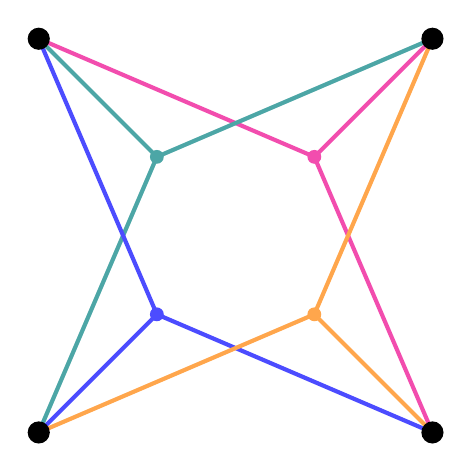
\begin{tikzpicture}[scale=1]
\coordinate (V1) at (0, 5);
\coordinate (V2) at (5, 5);
\coordinate (V3) at (5, 0);
\coordinate (V4) at (0, 0);
\coordinate (R0) at (3.500, 3.500);
\draw[line width=1.5pt, color=magenta!70!white] (R0) -- (V1);
\draw[line width=1.5pt, color=magenta!70!white] (R0) -- (V2);
\draw[line width=1.5pt, color=magenta!70!white] (R0) -- (V3);
\fill[color=magenta!70!white] (R0) circle (2.5pt);
\coordinate (R1) at (1.500, 3.500);
\draw[line width=1.5pt, color=teal!70!white] (R1) -- (V1);
\draw[line width=1.5pt, color=teal!70!white] (R1) -- (V2);
\draw[line width=1.5pt, color=teal!70!white] (R1) -- (V4);
\fill[color=teal!70!white] (R1) circle (2.5pt);
\coordinate (R2) at (1.500, 1.500);
\draw[line width=1.5pt, color=blue!70!white] (R2) -- (V1);
\draw[line width=1.5pt, color=blue!70!white] (R2) -- (V3);
\draw[line width=1.5pt, color=blue!70!white] (R2) -- (V4);
\fill[color=blue!70!white] (R2) circle (2.5pt);
\coordinate (R3) at (3.500, 1.500);
\draw[line width=1.5pt, color=orange!70!white] (R3) -- (V2);
\draw[line width=1.5pt, color=orange!70!white] (R3) -- (V3);
\draw[line width=1.5pt, color=orange!70!white] (R3) -- (V4);
\fill[color=orange!70!white] (R3) circle (2.5pt);
\fill[black] (V1) circle (4.0pt);
\fill[black] (V2) circle (4.0pt);
\fill[black] (V3) circle (4.0pt);
\fill[black] (V4) circle (4.0pt);
\end{tikzpicture}
    \caption{A complete $3$-graph on $4$ vertices.}
    \label{fig:complete_kgraph}
\end{figure}

\subsection{Partite $k$-graphs and the chromatic number}\label{subsec:partite}

We now introduce the notion of partite $k$-graphs.

\begin{definition} \label{def:partite}
    for an integer $p \geq k$, a $k$-graph $G = (V, E)$ is \emph{$p$-partite}
    if there exists a partition $V = V_1 \cup \dots \cup V_p$
    such that every edge $e \in E$ intersects every part $V_i$ in at most one vertex.
    We may write $G = (V_1, \dots, V_p; E)$ and say that
    $G$ is a partite $k$-graph on $V_1, \dots, V_p$.
\end{definition}

A different view of $p$-partite $k$-graphs is to think of them as vertex colored $k$-graphs,
in the following sense.

\begin{definition}
    A \emph{proper vertex coloring} of a $k$-graph $G = (V, E)$ in $p$ colors
    is a map $\chi: V \to [p]$ such that $\chi$ is injective on every edge.
    The elements $\chi^{-1}(i)$ for $1 \leq i \leq p$ are called the \emph{color classes} of $G$.
    We say that $G$ is \emph{$p$-vertex-colorable} or \emph{$p$-colorable}.
\end{definition}

The two notions are equivalent in the following sense.

\begin{proposition}
    A $k$-graph $G = (V, E)$ is $p$-partite if and only if
    there exists a vertex coloring of $G$ in $p$ colors.
    \begin{proof}
        Let $G = (V, E)$ be a $k$-graph.
        if $G$ is $p$-partite (say, $G = (V_1, \dots, V_p; E)$),
        then we can construct a vertex coloring of $G$ in $p$ colors
        by assigning to the vertices in $V_i$ the color $i$.
        The coloring is proper by Definition~\ref{def:partite}.
        Conversely, let $\chi: V \to [p]$ be a proper vertex coloring of $G$ in $p$ colors.
        Then the color classes form a partition of $V$ into $p$ sets where, by the injectivity of $\chi$ on edges,
        every edge $e \in E$ intersects every color class in at most one vertex.
    \end{proof}
\end{proposition}

To measure how easily colorable a $k$-graph is, we define the following.

\begin{definition}
    Let $G = (V, E)$ be a $k$-graph.
    The \emph{chromatic number} $\chi(G)$ of $G$ is the smallest integer $p \geq k$ such that
    $G$ is p-colorable (or, equivalently $p$-partite).
\end{definition}

If $G = (V_1, \dots, V_k; E)$ is a $k$-partite $k$-graph,
every edge intersects every part in exactly one vertex.
This means that we can identify the edges with a subset of $ V_1 \times \dots \times V_k$.
If it is clear from context, we may slightly abuse notation when talking about ordered and
unordered sets of vertices, as in the definition below.


\begin{definition} \label{def:complete_kpartite}
    A $k$-partite $k$-graph $G = (V_1, \dots, V_k; E)$ is \emph{complete}
    if $E = V_1 \times \dots \times V_k$.
    That is, if all $(v_1, \dots, v_k) \in V_1 \times \dots \times V_k$
    satisfy $\{v_1, \dots, v_k\} \in E$.
    We denote $G = \compdots{V_1}{V_k}$.
\end{definition}

In some cases, it is useful to generalize this notation to partite $k$-graphs
where the number of parts is different from $k$.

\begin{definition}
    Let $p \geq k \geq 1$.
    A $p$-partite $k$-graph $G = (V_1, \dots, V_p; E)$ is \emph{complete} if
    \[
        E = \bigcup_{\left\{i_1, \dots, i_k \right\} \in \binom{[p]}{k}} V_{i_1} \times \dots \times V_{i_k}.
    \]
    We denote $G = \compdotssuperindex{k}{V_1}{V_p}$.

\end{definition}

If $V_1, \dots, V_p$ and $W_1, \dots, W_p$ are disjoint sets
and $|V_i| = |W_i| = a_i$ for all $i$, then
\[
    \compdotssuperindex{k}{V_1}{V_p} \cong \compdotssuperindex{k}{W_1}{W_p}.
\]
An isomorphism is given by any bijection $f: V \to W$ (where $V=\cup_i V_i, W=\cup_i W_i$)
such that $f(V_i) = W_i$ for all $i$.
This allows us to talk, up to isomorphism, about \emph{the} complete $p$-partite $k$-graph
with part sizes $a_1, \dots, a_p$, which we denote by
\[
    \compdotssuperindex{k}{a_1}{a_p},
\]
or, in the $k$-partite case, by
\[
    K(a_1, \dots, a_k) = K^{(k)}(a_1, \dots, a_k).
\]

\begin{figure}[htbp]
    \centering
    % TikZ code for K^(3)(2, 2, 2) using predefined edge colors
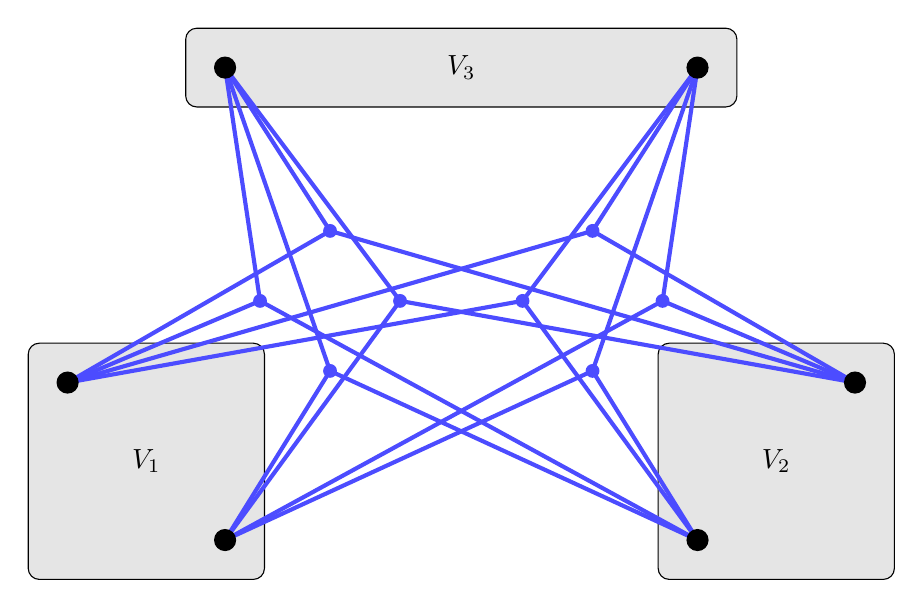
\begin{tikzpicture}[scale=1]
\draw[fill=gray!20, rounded corners] (-0.50, -0.50) rectangle (2.50, 2.50);
\node at (1.00, 1.00) [align=center] {$V_1$};
\draw[fill=gray!20, rounded corners] (7.50, -0.50) rectangle (10.50, 2.50);
\node at (9.00, 1.00) [align=center] {$V_2$};
\draw[fill=gray!20, rounded corners] (1.50, 5.50) rectangle (8.50, 6.50);
\node at (5.00, 6.00) [align=center] {$V_3$};
\coordinate (A1) at (2, 0);
\coordinate (A2) at (0, 2);
\coordinate (B1) at (8, 0);
\coordinate (B2) at (10, 2);
\coordinate (C1) at (2, 6);
\coordinate (C2) at (8, 6);
\coordinate (R0) at (3.333, 2.148);
\draw[line width=1.5pt, color=blue!70!white] (R0) -- (A1);
\draw[line width=1.5pt, color=blue!70!white] (R0) -- (B1);
\draw[line width=1.5pt, color=blue!70!white] (R0) -- (C1);
\fill[color=blue!70!white] (R0) circle (2.5pt);
\coordinate (R1) at (6.667, 2.148);
\draw[line width=1.5pt, color=blue!70!white] (R1) -- (A1);
\draw[line width=1.5pt, color=blue!70!white] (R1) -- (B1);
\draw[line width=1.5pt, color=blue!70!white] (R1) -- (C2);
\fill[color=blue!70!white] (R1) circle (2.5pt);
\coordinate (R2) at (4.222, 3.037);
\draw[line width=1.5pt, color=blue!70!white] (R2) -- (A1);
\draw[line width=1.5pt, color=blue!70!white] (R2) -- (B2);
\draw[line width=1.5pt, color=blue!70!white] (R2) -- (C1);
\fill[color=blue!70!white] (R2) circle (2.5pt);
\coordinate (R3) at (7.556, 3.037);
\draw[line width=1.5pt, color=blue!70!white] (R3) -- (A1);
\draw[line width=1.5pt, color=blue!70!white] (R3) -- (B2);
\draw[line width=1.5pt, color=blue!70!white] (R3) -- (C2);
\fill[color=blue!70!white] (R3) circle (2.5pt);
\coordinate (R4) at (2.444, 3.037);
\draw[line width=1.5pt, color=blue!70!white] (R4) -- (A2);
\draw[line width=1.5pt, color=blue!70!white] (R4) -- (B1);
\draw[line width=1.5pt, color=blue!70!white] (R4) -- (C1);
\fill[color=blue!70!white] (R4) circle (2.5pt);
\coordinate (R5) at (5.778, 3.037);
\draw[line width=1.5pt, color=blue!70!white] (R5) -- (A2);
\draw[line width=1.5pt, color=blue!70!white] (R5) -- (B1);
\draw[line width=1.5pt, color=blue!70!white] (R5) -- (C2);
\fill[color=blue!70!white] (R5) circle (2.5pt);
\coordinate (R6) at (3.333, 3.926);
\draw[line width=1.5pt, color=blue!70!white] (R6) -- (A2);
\draw[line width=1.5pt, color=blue!70!white] (R6) -- (B2);
\draw[line width=1.5pt, color=blue!70!white] (R6) -- (C1);
\fill[color=blue!70!white] (R6) circle (2.5pt);
\coordinate (R7) at (6.667, 3.926);
\draw[line width=1.5pt, color=blue!70!white] (R7) -- (A2);
\draw[line width=1.5pt, color=blue!70!white] (R7) -- (B2);
\draw[line width=1.5pt, color=blue!70!white] (R7) -- (C2);
\fill[color=blue!70!white] (R7) circle (2.5pt);
\fill[black] (A1) circle (4.0pt);
\fill[black] (A2) circle (4.0pt);
\fill[black] (B1) circle (4.0pt);
\fill[black] (B2) circle (4.0pt);
\fill[black] (C1) circle (4.0pt);
\fill[black] (C2) circle (4.0pt);
\end{tikzpicture}
    \caption{The complete 3-partite 3-graph $K(2, 2, 2)$, with parts $V_1, V_2, V_3$.}
    \label{fig:222}
\end{figure}

\begin{figure}[htbp]
    \centering
    % TikZ code for K^(2)(2, 2, 2) using predefined edge colors
\pgfdeclarelayer{background}
\pgfdeclarelayer{main}
\pgfsetlayers{background,main}
\begin{tikzpicture}[scale=0.8]
\begin{pgfonlayer}{background}
  \draw[fill=gray!20, rounded corners] (0.30, 0.30) rectangle (1.70, 3.70);
\end{pgfonlayer}
\node at (1.00, 2.00) [align=center] {$V_1$};
\begin{pgfonlayer}{background}
  \draw[fill=gray!20, rounded corners] (8.30, 0.30) rectangle (9.70, 3.70);
\end{pgfonlayer}
\node at (9.00, 2.00) [align=center] {$V_2$};
\begin{pgfonlayer}{background}
  \draw[fill=gray!20, rounded corners] (4.30, 5.30) rectangle (5.70, 8.70);
\end{pgfonlayer}
\node at (5.00, 7.00) [align=center] {$V_3$};
\coordinate (A1) at (1, 1);
\coordinate (A2) at (1, 3);
\coordinate (B1) at (9, 1);
\coordinate (B2) at (9, 3);
\coordinate (C1) at (5, 6);
\coordinate (C2) at (5, 8);
\draw[line width=1.5pt, color=magenta!60!white] (A1) -- (B1);
\draw[line width=1.5pt, color=magenta!60!white] (A1) -- (B2);
\draw[line width=1.5pt, color=magenta!60!white] (A2) -- (B1);
\draw[line width=1.5pt, color=magenta!60!white] (A2) -- (B2);
\draw[line width=1.5pt, color=teal!60!white] (A1) -- (C1);
\draw[line width=1.5pt, color=teal!60!white] (A1) -- (C2);
\draw[line width=1.5pt, color=teal!60!white] (A2) -- (C1);
\draw[line width=1.5pt, color=teal!60!white] (A2) -- (C2);
\draw[line width=1.5pt, color=orange!60!white] (B1) -- (C1);
\draw[line width=1.5pt, color=orange!60!white] (B1) -- (C2);
\draw[line width=1.5pt, color=orange!60!white] (B2) -- (C1);
\draw[line width=1.5pt, color=orange!60!white] (B2) -- (C2);
\begin{pgfonlayer}{main}
  \fill[black] (A1) circle (4.0pt);
  \fill[black] (A2) circle (4.0pt);
  \fill[black] (B1) circle (4.0pt);
  \fill[black] (B2) circle (4.0pt);
  \fill[black] (C1) circle (4.0pt);
  \fill[black] (C2) circle (4.0pt);
\end{pgfonlayer}
\end{tikzpicture}
    \caption{The complete 3-partite 2-graph $K^{(2)}(2, 2, 2)$, with parts $V_1, V_2, V_3$.}
    \label{fig:k2_222}
\end{figure}

Figure~\ref{fig:222} shows the complete $3$-partite $3$-graph
with $2$ vertices in each part, $K(2, 2, 2) = K^{(3)}(2, 2, 2)$.
In contrast, Figure~\ref{fig:k2_222} shows the complete $3$-partite $2$-graph
$K^{(3)}(2, 2, 2)$.

\subsection{Turán Problem for $k$-graphs}\label{subsec:turan}

Now we can state the \emph{forbidden subgraph problem} for $k$-graphs.
Informally, given a $k$-graph $G$, and an integer $n \geq |V(G)|$,
we want to find the smallest $M_0$ such that all $k$-graphs with $n$ vertices and $m > M_0$ edges
contain $G$ as a subgraph.

\begin{proposition} \label{prop:extremal}
    Let $G = (V, E)$ be a $k$-graph with nonempty edge set and $n \geq |V|$ be an integer.
    Then there exists an integer $M_0 = \ex{n}{G} \in \left[ 0, \binom{n}{k}\right)$ such that
    the condition
    \[
        \text{``All $k$-graphs with $n$ vertices and $m$ edges contain $G$ as a subgraph.''}
    \]
    is true for all $\binom{n}{k} \geq m > M_0$ and false for all $0 \leq m \leq M_0$.

    \begin{proof}
        Note that, if $M_0$ exists, clearly it is unique.
        Also, the condition is clearly false for $m = 0$ and
        true for $m = \binom{n}{k}$
        (the only graph $H$ with vertex set $W$, $|W|=n$ and $\binom{n}{k}$ edges
        is the one having all $k$-sets of vertices so any injective map $f: V \to W$
        is an embedding of $G$ in $H$).
        We only need to show that if the condition is true for $m$ then it is true for
        all $m' \geq m$.
        Suppose it is true for $m$ and let $m' \geq m$.
        Let $H = (W, F)$ be a $k$-graph with $n$ vertices and $m'$ edges.
        We can take $F' \subset F$ with $|F'| = m$.
        By hypothesis, the graph $H' = (W, F')$ contains $G$ as a subgraph,
        and the identity map in $W$ is an embedding of $H'$ in $H$:
        \[
            G \subset H' \subset H \implies G \subset H. \qedhere
        \]
    \end{proof}

\end{proposition}

\begin{definition}
    The integer $\ex{n}{G}$ defined in Proposition~\ref{prop:extremal}
    is called the \emph{extremal number} of $G$.
\end{definition}

\begin{remark}
    The extremal number $\ex{n}{G}$ is clearly invariant under isomorphism of $G$.
\end{remark}

There are very few $k$-graphs $G$ for which an exact formula for $\ex{n}{G}$ is known.
Of these, the most famous family of examples are the complete $2$-graphs $\completesuperindex{2}{r}$,
for which extremal numbers were first studied by Turán~\cite{Turan1941} in 1941.
The result is the following.

\begin{theorem}[Turán Theorem]
    \label{thm:turan}
    Let $r > 2$ be an integer and let $n \geq r$.
    Let $a_1, \dots, a_{r-1}$ be integers such that $a_1 + \dots + a_{r-1} = n$
    and $\lfloor n / (r-1) \rfloor \leq a_i \leq \lceil n / (r-1) \rceil$ for all $i$.
    Then
    \[
        \ex{n}{\completesuperindex{2}{r}} = \sum_{\{x, y\} \in \binom{[r-1]}{2}} a_x \cdot a_y
    \]
    Furthermore, if $G$ is a $2$-graph with $\ex{n}{\completesuperindex{2}{r}}$ edges
    and $G$ does not contain $K_r^{(2)}$ as a subgraph,
    then $G$ is a complete $(r-1)$-partite graph with part sizes $a_1, \dots, a_{r-1}$,
    that is,
    $G\cong \compdotssuperindex{2}{a_1}{a_{r-1}}$.
    
    \begin{proof}
        % TODO
    \end{proof}
\end{theorem}

% TODO Turán theorem, Erdős-Stone theorem, Erdos-Stone-Simonovits theorem, conjectures for uniformity 3


\subsection{Degenerate Turán Problems}\label{subsec:degenerate}

\begin{remark}
    All $k$-partite $k$-graphs with part sizes $b_1 \leq a_1, \dots, b_k \leq a_k$
    are contained in $\compdots{a_1}{a_k}$ as subgraphs.
    This lets us follow the same argument as in Proposition~\ref{prop:extremal}
    to define the following.
\end{remark}

\begin{definition}\label{def:zarankiewicz}
    Let $0 < t_1 \leq v_1, \dots, 0 < t_k \leq v_k$ be integers.
    Then the \emph{generalized Zarankiewicz number} $z(v_1, \dots, v_k; t_1, \dots, t_k)$
    is the largest integer $0 \leq z < \prod_i{ v_i}$ for which there exists a $k$-partite $k$-graph
    $H$ with part sizes $ |V_1| = v_1, \dots, |V_k| = v_k$ and $z$ edges
    such that no embedding $f$ of $\compdots{T_1}{T_k}$ with $|T_i| = t_i$ in it exists
    satisfying $f(T_i) \subset V_i$ for all $i$.
\end{definition}

From now on, every time we talk about embeddings from one $k$-partite $k$-graph
onto another we assume the condition $f(T_i) \subset V_i$.

\begin{remark}\label{rem:zar_vs_turan}
    Finding this number can help us upper bound the extremal number of $\compdots{t_1}{t_k}$ asymptotically:
    Assume that $H$ is a $\compdots{t_1}{t_k}$-free $n$-vertex $k$-graph with $m$ edges.
    pick $v_1, \dots, v_k$ such that $\sum_{i} v_i = n $ and $v_i \sim n/k $
    (For example $\lfloor n/k \rfloor \leq v_i \leq \lceil n/k \rceil$)
    Let $V_1, \dots, V_k$ be a random partition of $V(H)$ with $|V_i| = v_i$.
    for an edge $e \in E(H)$, the probability that $e$ is an edge in $\compdots{V_1}{V_k}$ is
    greater than
    \[k! \prod_i \frac{v_i}{n} \sim \frac{k!}{k^k},\]
    which is independent of $n$.
    Therefore, the expected number of edges satisfying this condition is a positive fraction of $m$.
    Applying the first moment method, we can conclude that
    \[
        \ex{n}{\compdots{t_1}{t_k}} = \bigO{\zaroversetdots{k}{\lceil n / k \rceil}{t_1}{t_k}}.
    \]

\end{remark}


The problem on finding the Zarankiewicz number was first posed by K. Zarankiewicz in 1951 for the
case of bipartite 2-graphs (that is, finding $z(u, w; s, t)$),
in terms of finding all-1 sub-matrices in a $0-1$ matrix.
An upper bound for it in the case $u=w, s=t$ was found by Kővari, Sós and Turán~\cite{Kovari1954} in 1954.
This was generalized to arbitrary complete
bipartite 2-graphs by C. Hyltén-Cavallius~\cite{Hylten1958} in 1958.
The result is stated and proved here for completeness.

\begin{theorem}\label{thm:kst}
    Let $0 < s \leq u$ and $0 < t \leq w$ be integers.
    Then 
    \[z(u, w; s, t) \leq (s - 1)^{1 / t}(w - t + 1)u^{1 - 1 / t} + (t - 1)u\]
    \begin{proof}
        Suppose that we have a bipartite graph $G = (U, W; E)$
        with $|U| = u$, $|W| = w$ and $|E| = z$ exceeding the bound stated above.
        Let us consider the set
        \[
            P = \left\{ (x, Y) \in U \times \binom{W}{t}
            \middle\vert\, x \in N_G(Y) \right\}.
        \]
        Counting on the first coordinate, we get
        \begin{equation} \label{eq:kst_p_lower}
            |P| =
            \mathlarger{\mathlarger{\sum}}_{x \in U} \binom{d_G(x)}{t} =
            \mathlarger{\mathlarger{\sum}}_{x \in U} \varphi(d_G(x)) \geq
            u  \mathlarger{\mathlarger{\sum}}_{x \in U} \varphi(z/u) =
            u \binom{z / u}{t},
        \end{equation}
        where we define
        \[
            \varphi(x) =
            \begin{cases}
                \binom{x}{t}, & \text{if } x \geq t - 1. \\
                0, & \text{otherwise.}
            \end{cases}
        \]
        The function $\varphi$ is convex, so we get the inequality in~\eqref{eq:kst_p_lower}
        as a consequence of Jensen's inequality.
        The other equalities come from the fact that $\varphi(d)$ agrees
        with $\binom{d}{t}$ for all integers $d \geq 0$;
        and that by our bound on $z$, $z \geq (t-1)u \implies z/u \geq t - 1$.

        If we had $s$ different elements of $P$ with the same second coordinate $T$,
        they would all necessarily have different first coordinates
        (say $S = \{x_1, \dots, x_s\}$).
        But now, by definition of $P$, for all $a \in S, b \in T$, we have $\{a, b\} \in E$.
        This would mean that the inclusion map from $ S \cup T$ to $U \cup W$ is an embedding of
        $K(s, t)$ in $G$, as described in Definition~\ref{def:zarankiewicz}.
        Supposing that this is not the case, by the averaging we get
        \begin{equation} \label{eq:kst_p_upper}
            |P| \leq (s - 1) \binom{w}{t}.
        \end{equation}
        Putting inequalities~\eqref{eq:kst_p_lower} and~\eqref{eq:kst_p_upper}
        together, we get
        \begin{equation} \label{eq:kst_chained}
            u \binom{z / u}{t} \leq (s - 1) \binom{w}{t}.
        \end{equation}
        Now, because we can see $E$ as a subset of $U \times W$,
        we get $z \leq uw \implies z/u \leq w$.
        We claim that this implies that
        \begin{equation} \label{eq:kst_binom}
            \frac{(z/u - (t - 1))^t}{\binom{z/u}{t}} \leq \frac{(w - (t - 1))^t}{\binom{w}{t}},
        \end{equation}
        because the function
        \[
            g(x) = \frac{(x - (t - 1))^t}{\binom{x}{t}}
        \]
        is increasing for $x \geq t - 1$.
        To see this, we expand the denominator into a product and absorb the $(x - (t - 1))^t$ factor.
        \begin{equation} \label{eq:g_expansion}
            g(x) = \prod_{i=0}^{t-1} (x-(t-1)) \frac{i+1}{x-i} = t! \prod_{i=0}^{t-1} \frac{x-(t-1)}{x-i}.
        \end{equation}
        Every factor in the product on the right side of~\eqref{eq:g_expansion} is increasing
        in $x$ for $x \geq t - 1 \geq i$, proving the claim.
        Multiplying inequalities~\eqref{eq:kst_chained} and~\eqref{eq:kst_binom} yields
        \[
            u \, (z/u - (t - 1))^t \leq (s - 1)(w - (t - 1))^t.
        \]
        Then, algebraic manipulation then gives
        \[
            z \leq (s - 1)^{1 / t}(w - t + 1)u^{1 - 1 / t} + (t - 1)u,
        \]
        In contradiction with our assumption. \qedhere
    \end{proof}

\end{theorem}

\begin{remark}
    Following Remark~\ref{rem:zar_vs_turan}, we can use this bound to get an upper bound on the extremal number of $K(s, t)$:
    \[
        \ex{n}{K(s, t)} =
        \bigO{(s - 1)^{1 / t}\left(\left\lceil\frac{n}{2}\right\rceil - t + 1\right)n^{1 - 1 / t} + (t - 1)\left\lceil\frac{n}{2}\right\rceil} =
        \bigO{n^{2 - 1 / t}}.
    \]
    Note that if $s < t$, we get the better bound $\bigO{n^{2 - 1 / s}}$ by interchanging the roles of $s$ and $t$.
\end{remark}

In 1964, Erdős~\cite{Erods1964} generalized this result to arbitrary complete partite $k$-graphs in the following theorem.

\begin{theorem}\label{thm:erdos64}
    For $k \geq 2$ and $2 \leq t \leq \frac{n}{k}$,
    $\ex{n}{\compoverset{k}{t}} = \bigO{n^{k - \frac{1}{t^{k-1}}}}$.
    \begin{proof}
        By Remark~\ref{rem:zar_vs_turan}, it suffices to show that
        \[
            z = \zaroverset{k}{w}{t} = \bigO{w^{k - \frac{1}{t^{k-1}}}}
        \]
        as $w \to \infty$.
        We prove this by induction on $k$.
        For $k=2$, this is obtained by setting $u = w$ and $s = t$ in Theorem~\ref{thm:kst}.
        For $k > 2$, suppose by way of contradiction that the theorem is false.
        For all ${w_0 \in \N}$, ${K \in \mathbb{R}^+}$, there exists a $k$-partite $k$-graph $G = (W_1, \dots, W_k; E)$ with part sizes
        $|W_i| = w \geq w_0$ and ${|E| \geq K w^{k - \frac{1}{t^{k-1}}}}$ such that no embedding of $\compoverset{k}{t}$ in it exists.
        Consider, for each set $T \in \binom{W_k}{t}$, the associated \text{$(k-1)$-link}
        \link{G}{T}{k-1}.
        We claim that it does not contain $\compoverset{k-1}{t}$ as a subgraph.
        If it did (say, $T_1 \times \dots \times T_{k-1} \in E(\link{G}{T}{k-1})$),
        then $T_1 \times \dots \times T_{k-1} \times T \in E$
        would contradict the assumption that $G$ does not contain $\compoverset{k}{t}$ as a subgraph.
        This means that
        \begin{equation} \label{eq:conditionlink}
            \link{G}{T}{k-1} \text{ has at most $z'$ edges for all } T \in \binom{W_k}{t},
        \end{equation}
        where
        \[
            z' = \zaroverset{k-1}{w}{t}.
        \]
        Now, consider the bipartite graph $G' = (U, W; E')$, where
        \begin{align*}
            U &= W_1 \times \dots \times W_{k-1}, \\
            W &= W_k, \\
            E' &= \{(X, y) \in V \times W \mid X \cup \{y\} \in E\}.
        \end{align*}
        Condition~\eqref{eq:conditionlink} is equivalent to saying that
        there is no embedding of $K(z' + 1, t)$ onto $G'$ respecting the respective partitions.
        Furthermore, $G'$ has the same number of edges as $G$.
        Finally, we invoke Theorem~\ref{thm:kst} with
        ${u = |U| = w^{k-1}}$ and
        ${s = z' + 1}$ to get
        \begin{equation} \label{eq:erdos64_induction}
            K w^{k - \frac{1}{t^{k-1}}} \leq
            |E| = |E'| \leq
            (z')^{1 / t}(w - t + 1)w^{(k-1)(1 - 1 / t)} + (t - 1)w^{k-1}.
        \end{equation}
        By the inductive hypothesis, for $w_0$ and $K'$ large enough, we can bound
        \begin{equation} \label{eq:erdos64prime}
            z' \leq K' w^{(k - 1) - \frac{1}{t^{k-2}}}.
        \end{equation}
        Substituting inequality~\eqref{eq:erdos64prime} into~\eqref{eq:erdos64_induction} and approximating yields
        \[
            K w^{k - \frac{1}{t^{k-1}}} \leq (K')^{1 / t} w^{k-\frac{1}{t^{k-1}}} + (t - 1)w^{k-1}.
        \]
        Combining like terms and picking $K > 2 (K')^{1 / t}$ gives
        \[
            \frac{1}{2}K w^{k - \frac{1}{t^{k-1}}} < (t - 1)w^{k-1},
        \]
        which we can rewrite as
        \begin{equation} \label{eq:erdos64_contradiction}
            \frac{1}{2}Kw^{1 - \frac{1}{t^{k-1}}} < (t - 1).
        \end{equation}
        This is a contradiction, because the right side of inequality~\eqref{eq:erdos64_contradiction}
        is constant in $w$, while the left side grows to infinity as $w$ increases.
    \end{proof}
\end{theorem}

This approach can be generalized to give a lower bound on the number of
copies of $\compdots{t_1}{t_k}$ in a $k$-partite $k$-graph $G$
with different part sizes~\cite{carvajal2024canonical},
therefore upper bounding all generalized Zarankiewicz numbers.

% TODO: probabilistic upper bound, algebraic upper bound, discussion

